\documentclass[8pt]{beamer}

% Beamer style
%\usetheme[secheader]{Madrid}
% \usetheme{CambridgeUS}
\useoutertheme{infolines}
\usecolortheme[rgb={0.65,0.15,0.25}]{structure}
% \usefonttheme[onlymath]{serif}
\beamertemplatenavigationsymbolsempty
%\AtBeginSubsection

% Packagesg
%\usepackage[french]{babel}
\usepackage[latin1]{inputenc}
\usepackage{color}
\usepackage{xspace}
\usepackage{enumerate}
\usepackage{dsfont, stmaryrd}
% \usepackage{amsmath, amsfonts, amssymb}
\usepackage{amsmath, amsfonts, amssymb, MnSymbol}
\usepackage{epsfig}
\usepackage{tikz}
\usepackage{url}
\usepackage{/home/robin/LATEX/Biblio/astats}
%\usepackage[all]{xy}
\usepackage{graphicx}

% Commands
% Maths
% \newtheorem{theorem}{Theorem}
% \newtheorem{definition}{Definition}
\newtheorem{proposition}{Proposition}
% \newtheorem{assumption}{Assumption}
% \newtheorem{algorithm}{Algorithm}
% \newtheorem{lemma}{Lemma}
% \newtheorem{remark}{Remark}
% \newtheorem{exercise}{Exercise}
% \newcommand{\propname}{Prop.}
% \newcommand{\proof}{\noindent{\sl Proof:}\quad}
% \newcommand{\eproof}{$\blacksquare$}

% \setcounter{secnumdepth}{3}
% \setcounter{tocdepth}{3}
\newcommand{\pref}[1]{\ref{#1} p.\pageref{#1}}
\newcommand{\qref}[1]{\eqref{#1} p.\pageref{#1}}

% Colors : http://latexcolor.com/
\definecolor{darkred}{rgb}{0.65,0.15,0.25}
\definecolor{darkgreen}{rgb}{0,0.4,0}
\definecolor{darkred}{rgb}{0.65,0.15,0.25}
\definecolor{amethyst}{rgb}{0.6, 0.4, 0.8}
\definecolor{asparagus}{rgb}{0.53, 0.66, 0.42}
\definecolor{applegreen}{rgb}{0.55, 0.71, 0.0}
\definecolor{awesome}{rgb}{1.0, 0.13, 0.32}
\definecolor{blue-green}{rgb}{0.0, 0.87, 0.87}
\definecolor{red-ggplot}{rgb}{0.52, 0.25, 0.23}
\definecolor{green-ggplot}{rgb}{0.42, 0.58, 0.00}
\definecolor{purple-ggplot}{rgb}{0.34, 0.21, 0.44}
\definecolor{blue-ggplot}{rgb}{0.00, 0.49, 0.51}

% Commands
\newcommand{\backupbegin}{
   \newcounter{finalframe}
   \setcounter{finalframe}{\value{framenumber}}
}
\newcommand{\backupend}{
   \setcounter{framenumber}{\value{finalframe}}
}
\newcommand{\emphase}[1]{\textcolor{darkred}{#1}}
\newcommand{\comment}[1]{\textcolor{gray}{#1}}
\newcommand{\paragraph}[1]{\textcolor{darkred}{#1}}
\newcommand{\refer}[1]{{\small{\textcolor{gray}{{\cite{#1}}}}}}
\newcommand{\Refer}[1]{{\small{\textcolor{gray}{{[#1]}}}}}
\newcommand{\goto}[1]{{\small{\textcolor{blue}{[\#\ref{#1}]}}}}
\renewcommand{\newblock}{}

\newcommand{\tabequation}[1]{{\medskip \centerline{#1} \medskip}}
% \renewcommand{\binom}[2]{{\left(\begin{array}{c} #1 \\ #2 \end{array}\right)}}

% Variables 
\newcommand{\Abf}{{\bf A}}
\newcommand{\Beta}{\text{B}}
\newcommand{\Bcal}{\mathcal{B}}
\newcommand{\Bias}{\xspace\mathbb B}
\newcommand{\Cor}{{\mathbb C}\text{or}}
\newcommand{\Cov}{{\mathbb C}\text{ov}}
\newcommand{\cl}{\text{\it c}\ell}
\newcommand{\Ccal}{\mathcal{C}}
\newcommand{\cst}{\text{cst}}
\newcommand{\Dcal}{\mathcal{D}}
\newcommand{\Ecal}{\mathcal{E}}
\newcommand{\Esp}{\xspace\mathbb E}
\newcommand{\Espt}{\widetilde{\Esp}}
\newcommand{\Covt}{\widetilde{\Cov}}
\newcommand{\Ibb}{\mathbb I}
\newcommand{\Fcal}{\mathcal{F}}
\newcommand{\Gcal}{\mathcal{G}}
\newcommand{\Gam}{\mathcal{G}\text{am}}
\newcommand{\Hcal}{\mathcal{H}}
\newcommand{\Jcal}{\mathcal{J}}
\newcommand{\Lcal}{\mathcal{L}}
\newcommand{\Mt}{\widetilde{M}}
\newcommand{\mt}{\widetilde{m}}
\newcommand{\Nbb}{\mathbb{N}}
\newcommand{\Mcal}{\mathcal{M}}
\newcommand{\Ncal}{\mathcal{N}}
\newcommand{\Ocal}{\mathcal{O}}
\newcommand{\pt}{\widetilde{p}}
\newcommand{\Pt}{\widetilde{P}}
\newcommand{\Pbb}{\mathbb{P}}
\newcommand{\Pcal}{\mathcal{P}}
\newcommand{\Qcal}{\mathcal{Q}}
\newcommand{\qt}{\widetilde{q}}
\newcommand{\Rbb}{\mathbb{R}}
\newcommand{\Sbb}{\mathbb{S}}
\newcommand{\Scal}{\mathcal{S}}
\newcommand{\st}{\widetilde{s}}
\newcommand{\St}{\widetilde{S}}
\newcommand{\Tcal}{\mathcal{T}}
\newcommand{\todo}{\textcolor{red}{TO DO}}
\newcommand{\Ucal}{\mathcal{U}}
\newcommand{\Un}{\math{1}}
\newcommand{\Vcal}{\mathcal{V}}
\newcommand{\Var}{\mathbb V}
\newcommand{\Vart}{\widetilde{\Var}}
\newcommand{\Zcal}{\mathcal{Z}}

% Symboles & notations
\newcommand\independent{\protect\mathpalette{\protect\independenT}{\perp}}\def\independenT#1#2{\mathrel{\rlap{$#1#2$}\mkern2mu{#1#2}}} 
\renewcommand{\d}{\text{\xspace d}}
\newcommand{\gv}{\mid}
\newcommand{\ggv}{\, \| \, }
% \newcommand{\diag}{\text{diag}}
\newcommand{\card}[1]{\text{card}\left(#1\right)}
\newcommand{\trace}[1]{\text{tr}\left(#1\right)}
\newcommand{\matr}[1]{\boldsymbol{#1}}
\newcommand{\matrbf}[1]{\mathbf{#1}}
\newcommand{\vect}[1]{\matr{#1}} %% un peu inutile
\newcommand{\vectbf}[1]{\matrbf{#1}} %% un peu inutile
\newcommand{\trans}{\intercal}
\newcommand{\transpose}[1]{\matr{#1}^\trans}
\newcommand{\crossprod}[2]{\transpose{#1} \matr{#2}}
\newcommand{\tcrossprod}[2]{\matr{#1} \transpose{#2}}
\newcommand{\matprod}[2]{\matr{#1} \matr{#2}}
\DeclareMathOperator*{\argmin}{arg\,min}
\DeclareMathOperator*{\argmax}{arg\,max}
\DeclareMathOperator{\sign}{sign}
\DeclareMathOperator{\tr}{tr}
\newcommand{\ra}{\emphase{$\rightarrow$} \xspace}

% Hadamard, Kronecker and vec operators
\DeclareMathOperator{\Diag}{Diag} % matrix diagonal
\DeclareMathOperator{\diag}{diag} % vector diagonal
\DeclareMathOperator{\mtov}{vec} % matrix to vector
\newcommand{\kro}{\otimes} % Kronecker product
\newcommand{\had}{\odot}   % Hadamard product

% TikZ
\newcommand{\nodesize}{2em}
\newcommand{\edgeunit}{2.5*\nodesize}
\newcommand{\edgewidth}{1pt}
\tikzstyle{node}=[draw, circle, fill=black, minimum width=.75\nodesize, inner sep=0]
\tikzstyle{square}=[rectangle, draw]
\tikzstyle{param}=[draw, rectangle, fill=gray!50, minimum width=\nodesize, minimum height=\nodesize, inner sep=0]
\tikzstyle{hidden}=[draw, circle, fill=gray!50, minimum width=\nodesize, inner sep=0]
\tikzstyle{hiddenred}=[draw, circle, color=red, fill=gray!50, minimum width=\nodesize, inner sep=0]
\tikzstyle{observed}=[draw, circle, minimum width=\nodesize, inner sep=0]
\tikzstyle{observedred}=[draw, circle, minimum width=\nodesize, color=red, inner sep=0]
\tikzstyle{eliminated}=[draw, circle, minimum width=\nodesize, color=gray!50, inner sep=0]
\tikzstyle{empty}=[draw, circle, minimum width=\nodesize, color=white, inner sep=0]
\tikzstyle{blank}=[color=white]
\tikzstyle{nocircle}=[minimum width=\nodesize, inner sep=0]

\tikzstyle{edge}=[-, line width=\edgewidth]
\tikzstyle{edgebendleft}=[-, >=latex, line width=\edgewidth, bend left]
\tikzstyle{edgebendright}=[-, >=latex, line width=\edgewidth, bend right]
\tikzstyle{lightedge}=[-, line width=\edgewidth, color=gray!50]
\tikzstyle{lightedgebendleft}=[-, >=latex, line width=\edgewidth, bend left, color=gray!50]
\tikzstyle{lightedgebendright}=[-, >=latex, line width=\edgewidth, bend right, color=gray!50]
\tikzstyle{edgered}=[-, line width=\edgewidth, color=red]
\tikzstyle{edgebendleftred}=[-, >=latex, line width=\edgewidth, bend left, color=red]
\tikzstyle{edgebendrightred}=[-, >=latex, line width=\edgewidth, bend right, color=red]

\tikzstyle{arrow}=[->, >=latex, line width=\edgewidth]
\tikzstyle{arrowbendleft}=[->, >=latex, line width=\edgewidth, bend left]
\tikzstyle{arrowbendright}=[->, >=latex, line width=\edgewidth, bend right]
\tikzstyle{arrowred}=[->, >=latex, line width=\edgewidth, color=red]
\tikzstyle{arrowbendleftred}=[->, >=latex, line width=\edgewidth, bend left, color=red]
\tikzstyle{arrowbendrightred}=[->, >=latex, line width=\edgewidth, bend right, color=red]
\tikzstyle{arrowblue}=[->, >=latex, line width=\edgewidth, color=blue]
\tikzstyle{dashedarrow}=[->, >=latex, dashed, line width=\edgewidth]
\tikzstyle{dashededge}=[-, >=latex, dashed, line width=\edgewidth]
\tikzstyle{dashededgebendleft}=[-, >=latex, dashed, line width=\edgewidth, bend left]
\tikzstyle{lightarrow}=[->, >=latex, line width=\edgewidth, color=gray!50]


% Directory
\newcommand{\fignet}{/home/robin/RECHERCHE/RESEAUX/EXPOSES/FIGURES}
\newcommand{\figtree}{/home/robin/RECHERCHE/BAYES/VBEM-IS/VBEM-IS.git/Data/Tree/Fig}
\newcommand{\figbayes}{/home/robin/RECHERCHE/BAYES/EXPOSES/FIGURES}
\newcommand{\figeco}{/home/robin/RECHERCHE/ECOLOGIE/EXPOSES/FIGURES}
\newcommand{\figStR}{/home/robin/RECHERCHE/BAYES/PLNsampling/Paper/Figures}

%====================================================================
%====================================================================

%====================================================================
%====================================================================
\begin{document}
%====================================================================
%====================================================================

%====================================================================
\title[Improving variational inference]{Improving the variational inference of latent variable models in ecology}

\author[S. Robin]{S. Robin \\ ~\\
    Joint work with S. Donnet and J. Stoehr
  }

\institute[]{\small Sorbonne universit\'e \\ 
Laboratoire de Probabilit\'es, Statistique et Mod\'elisation (LPSM) \\ ~ \\ ~}

\date[Feb.'25, UVSQ]{
Mod\'elisation, analyse statistique, et applications en \'ecologie et climatologie}

%====================================================================
%====================================================================
\maketitle
%====================================================================

%====================================================================
%====================================================================
\section{Latent variable models in ecology}
\frame{\frametitle{Outline} \tableofcontents[currentsection]}
%====================================================================
\frame{\frametitle{Latent variable models in ecology}

  \paragraph{Latent  ('hidden', 'unobserved', ...) variables} are widely used in statistical ecology  \refer{PeG22b} to 
  \begin{itemize}
    \setlength{\itemsep}{.5\baselineskip}
    \item account for heterogeneity (species clustering, over-dispersion or 'excess' of zeros in population sizes), 
    \item encode dependency (due to space, genetics, ...), 
    \item represent a 'true' signal, observed with noise (animal movement), 
    \item ...
  \end{itemize}

  \bigskip \bigskip \pause
  \paragraph{Statistical perspective.} 
  \begin{itemize}
    \setlength{\itemsep}{.5\baselineskip}
    \item Number of latent variables $\simeq$ number of observed variables.
    \item Inference of the model parameters much easier if they were observed.
  \end{itemize}

}

%====================================================================
\frame{\frametitle{Joint species distribution models}

  \paragraph{Aim.} 
  Describe/understand the relationships that living species share with each other and with their environment (biogeography, community ecology). 

  \bigskip \bigskip \pause 
  \paragraph{Species distribution models.} 
  $n$ sites, $x_i =$ vector of environmental descriptors for site $i$, $Y_i =$ number of individual from the species of interest observed in site $i$:
  $$
  Y_i \sim \Fcal(\cdot; x_i, \beta).
  $$
  $\to$ Generalized linear (mixed) model \refer{ElL09,ZIW09}

  \bigskip \bigskip \pause
  \paragraph{Joint species distribution models.} 
  Same, but $Y_i = (Y_{i1}, \dots Y_{ip}) =$ vector of counts for $p$ species of interest observed in site $i$:
  $$
  Y_i \sim \Fcal_p(\cdot; x_i, \beta, \Sigma)
  $$
  $\to$ Multivariate generalized linear mixed model  \refer{WBO15,OvA20}
  
}

%====================================================================
\frame{\frametitle{Poisson log-normal model}

  \bigskip
  \paragraph{A joint species distribution model:} 
  Poisson-log normal distribution \refer{AiH89,CMR21}
  \begin{align*}
    & \text{in each site $i = 1 \dots n$:} & 
    \emphase{Z_i} & \sim \Ncal_p(0, \emphase{\Sigma}) \\
    & \text{for each specie $j = 1 \dots p$:} &
    Y_{ij} \mid Z_{ij} & \sim \Pcal(\exp(x_i^\top \emphase{\beta_j} + Z_{ij}))
  \end{align*} \pause
  \begin{itemize}
    \item $\beta_j =$ effects of the environmental covariates on species $j$ (\emphase{\sl abiotic} interactions)
    \item $\Sigma =$ between-species covariance matrix  (\emphase{\sl biotic} interactions)
  \end{itemize}

  \bigskip \bigskip \pause
  \paragraph{Fish species from the Barents sea.} 
  $n = 89$, $p = 30$, $d = 4$ covariates
  $$
  \begin{tabular}{ccc}
    Covariate effects & 
    Correlation induced & 
    Between species \\
    $\widehat{B}$ & 
    by the environment & 
    correlation  $\widehat{\Sigma}$ \\
    \includegraphics[width=.25\textwidth, trim=20 20 50 20, clip=]{\figeco/BarentsFish-coeffAll-woIntercept} & 
    \includegraphics[width=.25\textwidth, trim=20 20 50 20, clip=]{\figeco/BarentsFish-corrPred} & 
    \includegraphics[width=.25\textwidth, trim=20 20 50 20, clip=]{\figeco/BarentsFish-corrAll}
  \end{tabular}
  $$
}

%====================================================================
\frame{\frametitle{Species interaction networks}

  \paragraph{Aim.} 
  Understand the organization of species interactions, viewed as a network:
  \begin{itemize}
    \item trophic (who-eats-who; unipartite, directed), 
    \item plant-pollinator, host-parasites (bipartite), 
    \item number of shared parasites (unipartite, un-oriented, weighted), 
    \item ....
  \end{itemize}

  \bigskip \bigskip \pause
  \paragraph{Network model.} $n$ species, $x_i =$ vector of covariates for species $i$, $x_{ij}$ vector of covariates for the pair of species $(i, j)$, $Y_{ij} =$ interaction between species $i$ and $j$:
  $$
  Y = (Y_{ij})_{i, j = 1 \dots n} \sim \Fcal(\cdot; (x_i)_{i = 1 \dots n}, (x_{ij})_{i, j = 1 \dots n}, \theta).
  $$
  $\to$ Exponential random graph models (ERGM: \refer{HHB08}), Block-models \refer{HoL79,GoN03} (review: \refer{MaR14})
  
}

%====================================================================
\frame{\frametitle{Stochastic block-model}

  \bigskip
  \paragraph{A network model:} 
  Stochastic block-model with covariates \refer{MRV10}
  \begin{align*}
    & \text{For each species $i = 1 \dots n$:} & 
    \emphase{Z_i} & \sim \Mcal_K(0, \emphase{\pi}) \\
    & \text{For each species pair $(i, j)$:} &
    Y_{ij} \mid Z_i = q, Z_j = \ell & \sim \Pcal(\exp(\emphase{\alpha_{q\ell}} + x_{ij}^\top \emphase{\beta}))
  \end{align*} 
  \begin{itemize}
    \item $\pi_q =$ proportion of species belonging to group $k$ (\emphase{\sl node clustering})
    \item $\alpha_{q\ell}=$ group effect on the interaction intensity
    \item $\beta =$ effect of the covariates on the interaction intensity
  \end{itemize}
  
  \bigskip \bigskip \pause
  \paragraph{Tree interactions.} 
  $n = 51$ species, $Y_{ij} = \#$ common parasites \refer{VPD08}, $d = 3$ covariates
  $$
  \begin{tabular}{ccc}
    Observed adjacency matrix & Clustered network ($Q=4$) & Covariate effects \\
    \begin{tabular}{c}
    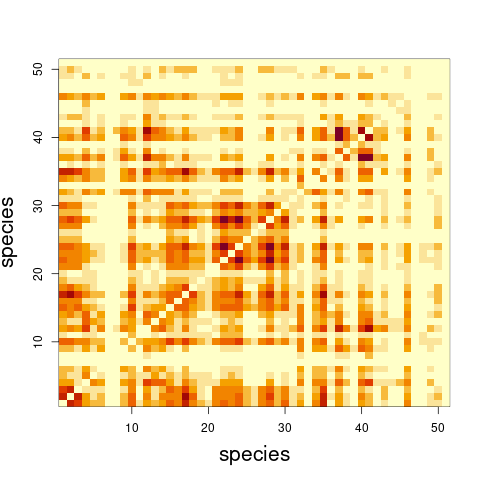
\includegraphics[width=.25\textwidth, trim=0 0 50 20, clip=]{\figbayes/FigUVSQ-Tree-Adjacency} 
    \end{tabular}
    & 
    \begin{tabular}{c}
    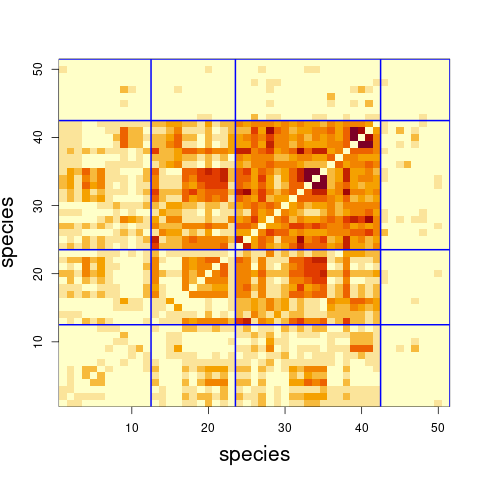
\includegraphics[width=.25\textwidth, trim=0 10 50 20, clip=]{\figbayes/FigUVSQ-Tree-ClustAdjacency-Covar}
    \end{tabular}
    &
    \begin{tabular}{l}
      $\widehat{\beta}_{\text{Gen}} = -0.413$ \\ ~ \\
      $\widehat{\beta}_{\text{Geo}} = -0.355$ \\ ~ \\
      $\widehat{\beta}_{\text{Tax}} = +0.036$
    \end{tabular}
  \end{tabular}
  $$
}

%====================================================================
%====================================================================
\section{From EM to Variationnal EM}
\frame{\frametitle{Outline} \tableofcontents[currentsection]}
%====================================================================
\frame{\frametitle{Maximum likelihood with latent variables}

  \paragraph{Latent variable model.} Three ingredients:
  \begin{enumerate}
    \item $\theta =$ parameter set:
    $$
    \text{PLN:} \theta = (B, \Sigma) \qquad \qquad \text{SBM:} \theta = (\pi, \alpha, \beta)
    $$
    \item $Z =$ set of latent variables:
    $$
    Z \sim p_\theta(Z)
    $$
    \item $Y =$ set of observed variables:
    $$
    Y \sim p_\theta(Y \mid Z)
    $$
  \end{enumerate}

  \bigskip \bigskip \pause
  \paragraph{Maximum likelihood inference.} Estimate $\theta$ with
  $$
  \widehat{\theta}
  = \argmax_\theta \log p_\theta(Y) 
  = \argmax_\theta \; \log \underset{\text{\normalsize Most often intractable}}{\underbrace{\int p_\theta(Y \mid z) p_\theta(z) \d z}} 
  $$

}

%====================================================================
\frame{\frametitle{EM algorithm}

  \paragraph{Expectation-Maximisation algorithm \refer{DLR77}.} $\theta^{(h)} =$ current value of the estimate,
  \begin{itemize}
    \item \emphase{E} step: Evaluate
    $$
    Q(\theta \mid \theta^{(h)}) := \Esp_{\theta^{(h)}}\left[\emphase{\log p_\theta(Y, Z)} \mid Y\right]
    $$
    \item \emphase{M} step: Update
    $$
    \theta^{(h+1)} = \argmax_\theta Q(\theta \mid \theta^{(h)})
    $$
  \end{itemize}
  $\to$ The log-likelihood increases at each step: $\log p_{\theta^{(h+1)}}(Y) \geq \log p_{\theta^{(h)}}(Y)$ .
  
  \bigskip \bigskip \pause
  \paragraph{Critical step = E step:} Requires to determine the conditional distribution
  $$
  p_\theta(Z \mid Y),
  $$
  or at least some of its moments.

  
  \bigskip \bigskip \pause
  \paragraph{Problem.} $p_\theta(Z \mid Y)$ is itself intractable for many models, including PLN and SBM
}

%====================================================================
\frame{\frametitle{Variational EM (VEM) algorithm}

  \paragraph{Principle \refer{WaJ08,BKM17}.} Replace the E step with an approximation step, i.e.
  \begin{itemize}
    \item Choose a class $\Qcal$ of approximate (parametric) distributions
    \item Choose divergence measure $D[q \| p]$ (e.g. $KL[q \| p]$)
    \item \emphase{VE} step :
    $$
    q^{(h+1)} = \argmin_{q \in \Qcal} D\left[q(Z) \| p_{\theta^{(h)}}(Z \mid Y)\right]
    $$
    \item \emphase{M} step :
    $$
    \theta^{(h+1)} = \argmax_\theta \Esp_{\emphase{q^{(h+1)}}}\left[\log p_\theta(Y, Z)\right]
    $$
  \end{itemize}
  $\to$ If $D = KL$, a lower bound of $\log p_\theta(Y)$ ('ELBO') increases at each step

  \bigskip \bigskip \pause
  \textcolor{gray}{\paragraph{Remark:} A Bayesian version of it exists (Variational Bayes EM = VBEM).}

  \bigskip
  \paragraph{Pros:} Reasonably easy to implement, fast, empirically accurate
  
  \bigskip \pause
  \paragraph{Cons:} Few theoretical guaranties \refer{CDP12,BCC13,MaM15}, does not enjoy the general properties of maximum likelihood (consistency, asymptotic normality, etc.) 
  \begin{itemize}
   \item No measure of uncertainty (\emphase{no test or confidence interval}) 
   \item Can we build upon variational inference to achieve 'genuine' statistical inference?
  \end{itemize}
  

}

%====================================================================
%====================================================================
\section{Ecological networks: Stochastic block-model }
\frame{\frametitle{Outline} \tableofcontents[currentsection]}
%====================================================================
\frame{\frametitle{Variational EM (VEM) for the stochastic block-model}

  \paragraph{Model.} 
  $n$ species
  \begin{align*}
    & \text{Species $i$:} & 
    Z_i & \sim \Mcal_K(0, \pi) 
    & & \text{(group membership)} \\
    & \text{Pair $(i, j)$:} &
    Y_{ij} \mid Z_i = q, Z_j = \ell & \sim \Pcal(e^{\emphase{\alpha_{q\ell}} + x_{ij}^\top \beta})
    & & \text{(observed interactions)}
  \end{align*} 

  \begin{tabular}{cc}
    \hspace{-.04\textwidth}
    \begin{tabular}{p{.75\textwidth}}
      \bigskip 
      \onslide+<2->{
      \paragraph{No EM.} 
      The $Z_i$'s are marginally independent, but are dependent conditional on the $Y_{ij}$'s.
      }

      \onslide+<3>{
      \bigskip \bigskip 
      \paragraph{Variational EM.} 'Mean-field' approximation \refer{GoN03,DPR08,MRV10}
      $$
      q(Z) = \prod_{i=1}^n q_i(Z_i)
      $$
      }
    \end{tabular}
    &
    \hspace{-.04\textwidth}
    \begin{tabular}{p{.25\textwidth}}
      \onslide+<2->{
      \begin{tikzpicture}
        \node[hidden] (Zi) at (0, 0) {$Z_i$};
        \node[hidden] (Zj) at (1.5, 0) {$Z_j$};
        \node[observed] (Yij) at (0.75, -1*\edgeunit) {$Y_{ij}$};
        \draw[arrow] (Zi) -- (Yij);
        \draw[arrow] (Zj) -- (Yij);
        \draw[-, line width=\edgewidth, color=gray, dashed] (Zi) -- (Zj);
      \end{tikzpicture}
      \vspace{0.25\textheight} 
      }
    \end{tabular} 
  \end{tabular}

  \vspace{-.05\textheight}
  \onslide+<3>{
  \begin{itemize}
    \item Parameter estimate $\widehat{\theta} = (\widehat{\pi}, \widehat{\alpha}, \widehat{\beta})$, 
    \item Approximate membership probability $\widetilde{\tau}_{ik} = \qt\{Z_i = k\}$, 
    \item Lower bound $ELBO(\widehat{\theta}, \widetilde{\tau})$ (R packages \url{blockmodels} \refer{Leg16}, \url{sbm} \refer{BDL17})
  \end{itemize}
  }
}

%====================================================================
\frame{\frametitle{Toward genuine Bayesian inference \refer{DoR21}}
  
  \bigskip \pause
  \paragraph{Bayesian model.} 
  Hierarchical structure
  \begin{align*}
  \text{\emphase{prior:}} \quad
  \theta & \sim \emphase{p(\theta)} & 
  Z & \sim p(Z \mid \theta) & 
  Y & \sim p(Y \mid Z, \theta)
  \end{align*}
  {Prior for SBM:} $p(\theta) = \Dcal(\pi; a_0) \times \Ncal([\alpha \; \beta]; m_0, V_0)$. 
  
  \bigskip \bigskip
  \paragraph{Aim of the inference:} be able to sample from the joint \emphase{posterior $p(\theta, Z \mid Y)$}
  
  \bigskip 
  \begin{tabular}{cc}
    \hspace{-.04\textwidth}
    \begin{tabular}{p{.6\textwidth}}
      \onslide+<3->{\paragraph{Sequential Monte Carlo sampling.} \refer{DDJ06}}
      \begin{itemize}
      \onslide+<3->{\item $\textcolor{red}{p_0} = $ proposal, $\textcolor{blue}{p^*} = $ target posterior \\ ~ \\}
      \onslide+<4->{\item Intermediate distributions
      $$
      \textcolor{red}{p_0}, \; p_1, \; \dots, \; p_H = \textcolor{blue}{p^*}
      $$}
      \onslide+<4->{\item Iteratively: use $p_h$ to get a sample from $p_{h+1}$}
      \end{itemize}
    \end{tabular}
    & 
    \hspace{-.1\textwidth}
    \begin{tabular}{p{.35\textwidth}}
%       \vspace{.025\textwidth}
      \begin{overprint}
      \onslide<3> 
      \includegraphics[width=.35\textwidth]{\figbayes/FigVBEM-IS-PropTarget.pdf}
      \onslide<4> 
      \includegraphics[width=.35\textwidth]{\figbayes/FigVBEM-IS-Tempering.pdf}
      \end{overprint}
    \end{tabular}
  \end{tabular}

}

%====================================================================
\frame{\frametitle{Proposed sequential sampling strategy (1/2)}

  \paragraph{Distribution path:}  
    set $0 = \rho_0 < \rho_1 < \dots < \rho_{H-1} < \rho_H = 1$,
  \begin{align*}
     p_h(\theta, Z) & \propto p_0(\theta, Z)^{\emphase{{1-\rho_h}}} \; \times \; p(\theta, Z | Y)^{\emphase{{\rho_h}}} \\
%      \\
     & \propto p_0(\theta, Z) \; \times \; r(\theta, Z)^{\emphase{{\rho_h}}}, 
     & r(\theta, Z) & = \frac{\pi(\theta, Z) \ell(Y | \theta, Z)}{p_0(\theta, Z)}
  \end{align*}
  
  \bigskip \pause
  \paragraph{Sequential sampling.} At each step $h$, provide
  $$
  \Ecal_h = \{(\theta_h^m, Z_h^m, w_h^m)\}_{m = 1 \dots M} = \text{ weighted sample from } p_h
  $$
  with $w_0^m = 1$, $w_h^m = w_{h-1}^m \times r(\theta^m, Z^m)^{\rho_h - \rho_{h-1}}$

  \bigskip \bigskip \pause
  \paragraph{Tuning $\rho_h$.} 
  Because 
  $$
  p_h(\theta, Z) \propto p_{h-1}(\theta, Z) \; \times \; r(\theta, Z)^{\emphase{{\rho_h} - \rho_{h-1}}}, 
  $$
  $\rho_h$ can be tuned so to guaranty a sufficiently high effective sampling size (ESS\footnote{$\simeq$ Variance of the weights}).
  
}

%====================================================================
\frame{\frametitle{Proposed sequential sampling strategy (2/2)}

  \bigskip
  \paragraph{Initial proposal distribution $p_0$.} Use VEM outputs:
  $$
  \pt_0(\theta) =  \Dcal(\pi; \widetilde{a}_0) \times \Ncal([\alpha \; \beta]; \widetilde{m}_0, \widetilde{V}_0)
  $$
  with  $\widetilde{a}_0 = f(a_0, \emphase{\widetilde{\tau}_{VEM}})$, $\widetilde{m}_0 = f(m_0, \emphase{\widehat{\theta}_{VEM}})$ and $\widetilde{V}_0 = f(S_0, - \nabla_\theta^2 \emphase{ELBO(\widehat{\theta}_{VEM}, \qt_{VEM})})$.
  
  \bigskip \bigskip \pause
  \begin{tabular}{cc}
    \hspace{-.04\textwidth}    
    \begin{tabular}{p{.35\textwidth}}
      \paragraph{What do we gain?} Mostly time: \\
      ~ \\
      $p_0 = \pt_0$ rather than $p_0 =$ prior \\
      ~ \\
      $\Rightarrow$ reduced number of SMC steps
      ~ \\ ~ \\ ~ \\ ~ \\ ~ \\ 
%       \flushright{Synthetic data $\to$}
%       ~ \\ ~ \\
    \end{tabular}
    &
    \begin{tabular}{c}
      \hspace{-.05\textwidth}    
      Synthetic data \\
      \includegraphics[width=.5\textwidth, trim=5 0 5 00, clip=]{\figbayes/DoR21-Fig1-simu-rho} 
    \end{tabular}
  \end{tabular}

}

%====================================================================
\frame{\frametitle{Tree interaction network}

  \paragraph{Posterior distribution of $\beta$.} For $\widehat{K} = 4 = \argmax_K p(K \mid Y)$, after \emphase{26 SMC steps}:
  $$
  \begin{tabular}{ccc}
    taxonomy & geography & genetics \\
    \includegraphics[width=.3\textwidth, trim=0 30 10 50, clip=]{\figbayes/DoR21-Fig7-beta1} & 
    \includegraphics[width=.3\textwidth, trim=0 30 10 50, clip=]{\figbayes/DoR21-Fig7-beta2} & 
    \includegraphics[width=.3\textwidth, trim=0 30 10 50, clip=]{\figbayes/DoR21-Fig7-beta3} \\
    \multicolumn{3}{c}{\textcolor{orange}{variational $\pt_0(\beta \mid \widehat{K})$}, \quad  \textcolor{darkgreen}{posterior $\widehat{p}(\beta \mid Y, \widehat{K})$}, \quad \textcolor{purple}{$\widehat{p}(\beta \mid Y)$ averaged of $K$}}
  \end{tabular}
  $$

  \paragraph{Model selection.} 
  $
  \widehat{P}\{x = \text{(taxo., geo.)} \mid Y \} \simeq 70\%, \quad
  \widehat{P}\{x = \text{(taxo.)} \mid Y \} \simeq 30\%
  $
   
  \bigskip \pause
  \hspace{-.025\textwidth}
  \begin{tabular}{rrrr}
    \paragraph{Correlation between estimates.} 
    & $(\beta_1, \beta_2)$ & $(\beta_1, \beta_3)$ & $(\beta_2, \beta_3)$ \\
    $\pt_0(\beta)$    & $-0.012$ & $ 0.021$ & $ 0.318$ \\
    $\widehat{p}(\beta \mid Y)$ & $-0.274$ & $-0.079$ & $-0.088$
  \end{tabular} \\
  \bigskip
  + $p(Z \mid Y)$ going away from $\prod_i q_i(Z_i)$ \textcolor{gray}{see backup slides}.

}


%====================================================================
%====================================================================
\section{Species abundances: Poisson log-normal model}
\frame{\frametitle{Outline} \tableofcontents[currentsection]}
%====================================================================
\frame{\frametitle{Variational EM (VEM) for the Poisson log-normal model}

  \paragraph{Model.} 
  $n$ sites, $p$ species
  \begin{align*}
    & \text{in each site $i = 1 \dots n$:} & 
    \emphase{Z_i} & \sim \Ncal_p(0, \emphase{\Sigma}) &
    & (\text{latent vector}) \\
    & \text{for each species $j = 1 \dots p$:} &
    Y_{ij} \mid Z_{ij} & \sim \Pcal(\exp(x_i^\top \emphase{\beta_j} + Z_{ij})) &
    & (\text{observed abundances})
  \end{align*} 
  
  \bigskip \pause
  \paragraph{No EM.} 
  The $Z_i$'s are marginally Gaussian, but not Gaussian conditionally on the $Y_{ij}$'s \\
  (no close form for $p(Z \mid Y)$, even in one dimension)
  
  \bigskip \bigskip \pause
  \paragraph{Variational EM.} Gaussian approximation \refer{CMR18a}
  $$
  q(Z) = \prod_{i=1}^n \Ncal(Z_i; m_i, S_i)
  $$
  \begin{itemize}
  \item Parameter estimate $\widehat{\theta} = (\widehat{\Sigma}, \widehat{\beta})$, 
  \item Approximate conditional distribution $Z_i \mid Y_i \approx \Ncal(\widetilde{m}_i, \widetilde{S}_i)$, 
  \item Lower bound $ELBO(\widehat{\theta}, \widetilde{m}, \widetilde{S})$ (R package \url{PLNmodels})
  \end{itemize}
  
}

%====================================================================
\frame{\frametitle{Toward genuine maximum likelihood inference \refer{StR24}}

  \pause
  \paragraph{Monte Carlo EM.} \refer{CeD85} When $p(Z \mid Y)$ intractable:
  \begin{itemize}
    \item Monte Carlo E step: Sample $(Z^m)_{m = 1 \dots M} \overset{iid}{\sim} p_{\theta^{(h)}}(Z \mid Y)$, then estimate
    $$
    \widehat{Q}(\theta \mid \theta^{(h)}) := \frac1{M} \sum_{m=1}^M \log p_\theta(Y, Z^m)
    $$
    \item M step: Update
    $$
    \theta^{(h+1)} = \argmax_\theta \widehat{Q}(\theta \mid \theta^{(h)}) 
    $$
  \end{itemize}

  \bigskip \pause
  \paragraph{How to sample from $p_{\theta^{(h)}}(Z \mid Y)$?}
  Importance sampling:
  \begin{itemize}
   \item Sample $(Z^m)_{m = 1 \dots M} \overset{iid}{\sim} q^{(h)}(Z)$, $q^{(h)} =$ Gaussian proposal,
   \item Compute the non-normalized weights $\rho_m^{(h)} = p_{\theta^{(h)}}(Y, Z^m) \left/ q^{(h)}(Z^m)\right.$,
   \item \pause Estimate
    $$
    \widehat{Q}(\theta \mid \theta^{(h)}) := \sum_{m=1}^M \rho_m^{(h)} \log p_\theta(Y, Z^m) \; \left/ \; \sum_{m=1}^M \rho_m^{(h)} \right.,
    $$
  \end{itemize}

}

%====================================================================
\frame{\frametitle{Composite likelihood}

  \paragraph{Importance sampling has a poor efficiency\footnote{Measured in terms of ESS $\simeq$ variance of the weights}} in large dimension (say $p \geq 10, 15$) \\
  ~  
  $\to$ Need to reduce the sampling dimension

  \bigskip \pause
  \paragraph{Composite likelihood.} 
  \begin{itemize}
    \item Build $B$ overlapping blocks $\Ccal_1, \dots \Ccal_B$, each containing $k$ species, 
    \item Define the composite log-likelihood as
    $$
    \cl_\theta(Y) = \frac1B \sum_{b=1}^B \log p_\theta(Y^b), 
    \qquad
    \text{where} \quad 
    Y^b = [Y_{ij}]_{i = 1, \dots n, j \in \Ccal_b},
    $$
    \item \pause Then, the maximum composite likelihood estimator \refer{VRF11}
    $$
    \widehat{\theta}_{CL} = \argmax_\theta \cl_\theta(Y) 
    $$
    is consistent, asymptotically Gaussian with asymptotic variance given by
    \begin{align*}
      J(\theta) & = \Var_\theta[\nabla_\theta \cl_\theta(Y)], 
      \qquad \qquad 
      H(\theta) = - \Esp_\theta[\nabla^2_\theta \cl_\theta(Y)], \\
      \Var_\infty(\widehat{\theta}_{CL}) & = H^{-1}(\theta) J(\theta) H^{-1}(\theta).
    \end{align*} 
  \end{itemize}

}

%====================================================================
\frame{\frametitle{Proposed composite likelihood algorithm}

  \paragraph{Dealing with latent variables.}
  \begin{itemize}
    \item The latent variables $Z$ can be split in the same way as the observed abundances $Y$
    \item The EM algorithm applies to the composite log-likelihood (apply the EM decomposition within each block)
  \end{itemize}

  \bigskip \bigskip \pause
  \paragraph{Proposal for importance sampling.}
  \begin{itemize}
    \item Start with $q^{(1)}(Z) = \qt_{VEM}(Z)$
    \item Then update $q^{(h+1)}(Z)$ with the estimated mean and variance of $p_{\theta^{(h)}}(Z \mid Y)$.
  \end{itemize}

  \bigskip \bigskip \pause
  \paragraph{Building the blocks.} To guaranty the same precision for all estimates, one would ideally want that
  \begin{itemize}
    \item[$\beta_j$:] Each species $j$ belongs in the same number of blocks $\Ccal_1, \dots \Ccal_B$
    \item[$\sigma_{jj'}$:] Each pair of species $(j, j')$ appears in the same number of blocks 
    \item Same problem as the construction of a Balanced Incomplete Block Design\footnote{Not always possible: need to have $p \mid Bk$ and $p(p-1) \mid Bk(k-1)$}
  \end{itemize}

}

%====================================================================
\frame{\frametitle{Simulation study}

  \paragraph{Main aim.} Assess normality 
  \begin{itemize}
    \item Test statistic $(\widehat{\theta} -\theta^*) /\sqrt{\widehat{\Var}_\infty(\widehat{\theta})}$ for the regression coefficients
    \item Criterion = $p$-value of the Kolmogorov-Smirnov test for normality
  \end{itemize}
  
  \bigskip \bigskip \pause
  \paragraph{Results.} $100$ sites, $3$ covariates, $100$ simulations
  \newcommand{\lagSim}{50} \newcommand{\nISsim}{200} \newcommand{\nIterSim}{1000}
  \newcommand{\simulParms}{-nIter\nIterSim-lag\lagSim-nIS\nISsim}
  $$
  \begin{tabular}{cccc}
    7 species & 10 species & 20 species & 50 species \\
    \includegraphics[width=.2\textwidth, trim=10 10 25 25, clip=]{\figStR/PvalKS-score-n100-d3-p7-parm1\simulParms} & 
    \includegraphics[width=.2\textwidth, trim=10 10 25 25, clip=]{\figStR/PvalKS-score-n100-d3-p10-parm1\simulParms} & 
    \includegraphics[width=.2\textwidth, trim=10 10 25 25, clip=]{\figStR/PvalKS-score-n100-d3-p20-parm1\simulParms} &
    \includegraphics[width=.2\textwidth, trim=10 10 25 25, clip=]{\figStR/PvalKS-score-n100-d3-p50-parm1\simulParms}  
  \end{tabular}
  $$
  FL = full likelihood, CL$k$ = composite likelihood$(k)$, \\
  \medskip
  VEM = pseudo Fisher information,  JK = jackknife variance estimate of $\Var(\widehat{\theta}_{VEM})$

}

%====================================================================
\frame{\frametitle{Fish species in the Barents sea}

  \newcommand{\nIterEx}{10000} \newcommand{\lagEx}{50} \newcommand{\nISex}{200}
  \newcommand{\exampleParms}{-nIter\nIterEx-lag\lagEx-nIS\nISex}
  \newcommand{\nIterSel}{\nIterEx} \newcommand{\lagSel}{20} \newcommand{\nISsel}{\nISex}
  \newcommand{\selectParms}{-nIS\nISsel-nIter\nIterSel-lag\lagSel}
  
  \bigskip
  \paragraph{Comparison of the estimates.}
  $$
  \begin{tabular}{ccc}
    $\widehat{B}$ & $\widehat{\Sigma}$ & ESS (CL5) \\
    \includegraphics[width=.25\textwidth, trim=10 10 25 50, clip=]{\figStR/Barents\exampleParms-compBeta-cem5-all} & 
    \includegraphics[width=.25\textwidth, trim=10 10 25 50, clip=]{\figStR/Barents\exampleParms-compSigma-cem5-all} & 
    \includegraphics[width=.25\textwidth, trim=10 10 25 50, clip=]{\figStR/Barents\exampleParms-ESS-cem5}     
  \end{tabular}
  $$

  \pause
  \paragraph{Significance.}
  $$
  \begin{tabular}{ccc}
    $\widehat{B}$ & $\widehat{\Sigma}$ & $\text{cor}(\widehat{\Sigma})$ \\
    \includegraphics[width=.25\textwidth, trim=10 10 25 25, clip=]{\figStR/Barents\exampleParms-betaSignif-cem5} & 
    \includegraphics[width=.25\textwidth, trim=10 10 25 25, clip=]{\figStR/Barents\exampleParms-sigmaSignif-cem5} &
    \includegraphics[width=.25\textwidth, trim=10 10 25 25, clip=]{\figStR/Barents\exampleParms-corSigmaSignif-cem5}
  \end{tabular}  
  $$
}

%====================================================================
%====================================================================
\section{Discussion}
\frame{\frametitle{Outline} \tableofcontents[currentsection]}
%====================================================================
\frame{\frametitle{Discussion}

  \paragraph{Summary.}
  \begin{itemize}
    \setlength{\itemsep}{.75\baselineskip}
    \item Latent variable models are widely used in statistical ecology
    \item Maximum likelihood inference is often intractable \\
    $\to$ Variational inference = appealing alternative ... with few theoretical guaranties
    \item Monte Carlo approaches moves from variational inference toward genuine maximum likelihood or Bayesian inference
  \end{itemize}

  \bigskip \bigskip \pause
  \paragraph{Comments.}
  \begin{itemize}
    \setlength{\itemsep}{.75\baselineskip}
    \item Monte Carlo approaches as still computationally demanding
    \item ML-based variational inference (variational auto-encoders) may correspond to larger approximation class $\Qcal$, therefore to more flexible approximate distribution $\qt$, getting closer to genuine MLE
    \item More insights about the statistical properties of variational estimates are still needed
  \end{itemize}


}

%====================================================================
\backupbegin
%====================================================================

%====================================================================
\frame[allowframebreaks]{ \frametitle{References}
{\tiny
  \bibliography{/home/robin/Biblio/BibGene}
%   \bibliographystyle{/home/robin/LATEX/Biblio/astats}
  \bibliographystyle{alpha}
  }
}

%====================================================================
\frame{ \frametitle{Tree interaction network: dataset}

  
  $$
  \begin{tabular}{ccc}
    & Observed network & Adjacency matrix \\
    \begin{tabular}{p{0.24\textwidth}}
      $n = 51$ tree species \\ ~\\
      $d = 3$ edge covariates \\
      (distances) \\ ~\\
    \end{tabular}
    &
    \begin{tabular}{c}
    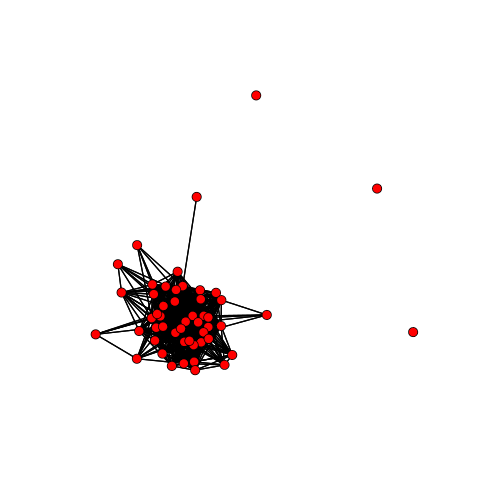
\includegraphics[width=.22\textwidth, trim=0 0 50 20, clip=]{\figbayes/FigUVSQ-Tree-Network} 
    \end{tabular}
    &
    \begin{tabular}{c}
    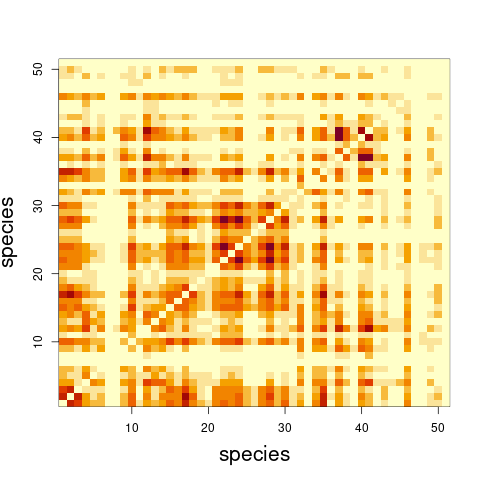
\includegraphics[width=.22\textwidth, trim=0 10 50 20, clip=]{\figbayes/FigUVSQ-Tree-Adjacency}
    \end{tabular}
  \end{tabular}
  $$

  \bigskip
  $$
  \begin{tabular}{ccccc}
    Genetic (log) & & Geographic & & Taxonomic \\
    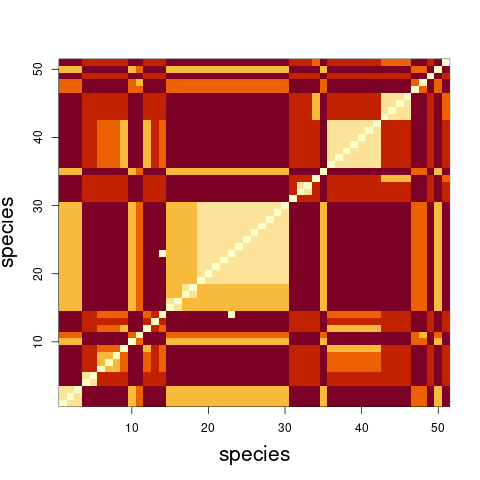
\includegraphics[width=.22\textwidth, trim=0 10 50 20, clip=]{\figbayes/FigUVSQ-Tree-GeneticDistance} &
    \qquad &
    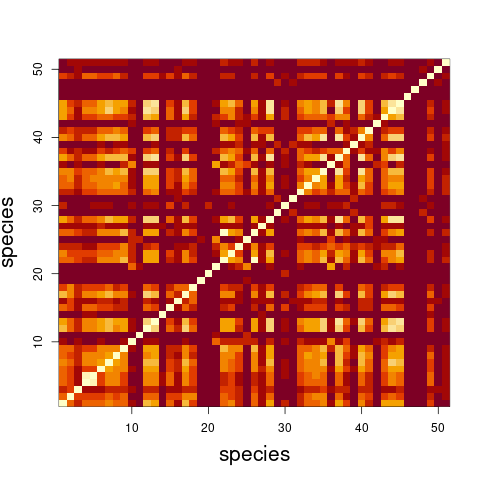
\includegraphics[width=.22\textwidth, trim=0 10 50 20, clip=]{\figbayes/FigUVSQ-Tree-GeographicDistance} & 
    \qquad &
    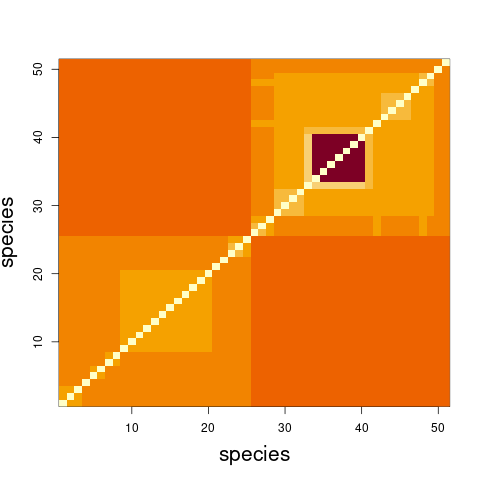
\includegraphics[width=.22\textwidth, trim=0 10 50 20, clip=]{\figbayes/FigUVSQ-Tree-TaxonomicDistance}
  \end{tabular}
  $$
}

%====================================================================
\frame{\frametitle{Tree interaction network: Sampling path \& choice of $K$}

  \paragraph{Full model.} All covariates

  \bigskip
  \begin{center}
    \begin{tabular}{ccc}
    Model selection & & Sampling path: $\rho_h$ \\
    \includegraphics[width=.3\textwidth]{\figbayes/DoR21-Fig7-logpY} &
    \qquad &
    \includegraphics[width=.3\textwidth]{\figbayes/DoR21-Fig7-rho} \\
    \textcolor{orange}{$J_K$}, \textcolor{darkgreen}{$\log (Y \mid K)$}, \textcolor{purple}{$\widetilde{ICL}(K)$} 
    \end{tabular}
  \end{center}
  
  \bigskip \bigskip
  \paragraph{Choosing the number of groups:} $\widehat{K} = \arg\max_K \widehat{p}(K \mid Y)$ 
  \begin{itemize}
    \item Different from $\arg\max_K \widetilde{ICL}(K)$ here.
  \end{itemize}
}

%====================================================================
\frame{\frametitle{Tree interaction network: Conditional dependence between the $Z_i$}

  The conditional dependency between the latent $Z_i$ can be measured at each sampling step by their mutual information
  $$
  MI = KL\left(\prod_i p_h(Z_i) \mid p_h(Z)\right).
  $$
  
  \bigskip 
  Part of the effort of the algorithm is dedicated to the recovery of this conditional dependency structure.
  $$
  \includegraphics[width=.3\textwidth]{\figbayes/DoR21-Fig7-MI} 
  $$
}
  
%====================================================================
\frame{ \frametitle{Tree interaction network: SBM node clustering}

  \paragraph{Clustered networks.} 
  $$
  \begin{tabular}{ccc}
    No covariate ($Q = 6$) & 3 covariates ($Q=4$) & Covariate effects \\
    \begin{tabular}{c}
    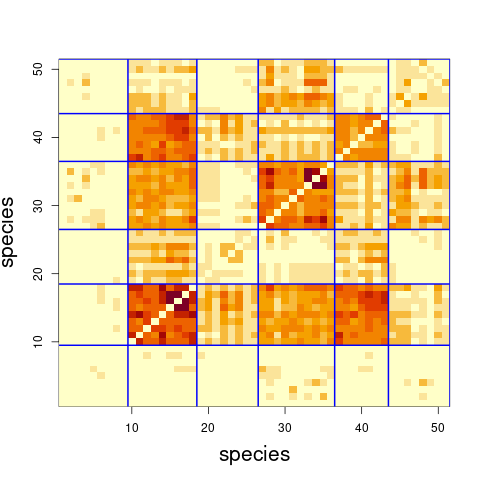
\includegraphics[width=.25\textwidth, trim=0 10 50 20, clip=]{\figbayes/FigUVSQ-Tree-ClustAdjacency-noCovar}
    \end{tabular}
    & 
    \begin{tabular}{c}
    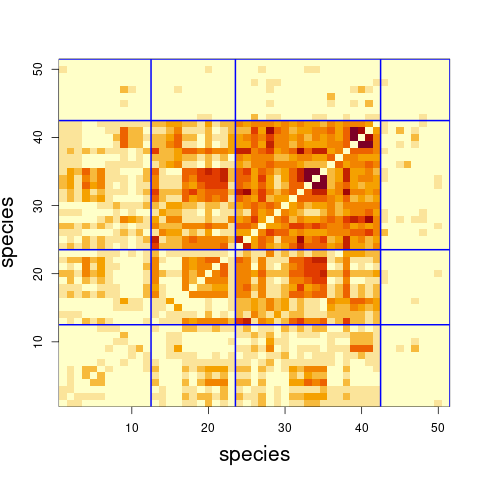
\includegraphics[width=.25\textwidth, trim=0 10 50 20, clip=]{\figbayes/FigUVSQ-Tree-ClustAdjacency-Covar}
    \end{tabular}
    &
    \begin{tabular}{l}
      $\widehat{\beta}_{\text{Gen}} = -0.413$ \\ ~ \\
      $\widehat{\beta}_{\text{Geo}} = -0.355$ \\ ~ \\
      $\widehat{\beta}_{\text{Tax}} = +0.036$
    \end{tabular}
  \end{tabular}
  $$

}

%====================================================================
\frame{\frametitle{Tree interaction network: residual structure}

  Between group interactions ($\alpha_{k\ell}$) = 'residuals' = not explained by the covariates.

  \pause
  \hspace{-.05\textwidth}
  \begin{tabular}{cc}
    \begin{tabular}{p{.4\textwidth}}
      \paragraph{'Graphon' representation.} \refer{LRO17} \\
      Group interactions encoded as
      $$
      \phi: [0, 1]^2 \mapsto \Rbb
      $$
      \begin{itemize}
       \item symmetric\footnote{with increasing marginal $\overline{\phi}(u) = \int \phi(u, v) \d v$ to ensure identifiability.}, 
       \item block-wise constant, 
       \item block width $= \pi_k$
       \item block height $= \alpha_{k\ell}$
      \end{itemize}
    \end{tabular}
    & 
    \begin{tabular}{p{.5\textwidth}}
      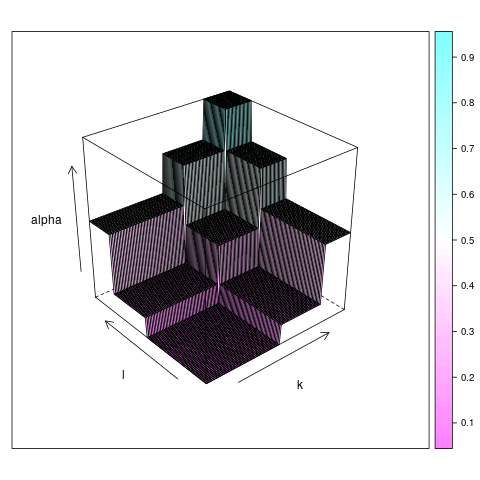
\includegraphics[trim=50 50 50 50, width=.5\textwidth, clip=T]{\fignet/FigGraphon-SBM-graphon-alpha}
    \end{tabular}
  \end{tabular}
  
%   \vspace{-.1\textheight}
  \pause 
  \paragraph{Same representation for all $K$.}
  $
  Y_{ij} | (U_i, U_j) \sim \Pcal\left(\exp(\phi(U_i, U_j) + x_{ij}^\top \beta \right)
  $
  
  }

%====================================================================
\frame{\frametitle{Tree interaction network: residual graphon}

%   \vspace{-.2\textheight}
  \hspace{-.04\textwidth}
  \begin{tabular}{cc}
    \begin{tabular}{p{.4\textwidth}}
      \paragraph{Residual graphon.} \\
      Each particle $\theta^m$ provides an estimate of $\phi^m(u, v)$ \\
      ~ \\
      ~ \\
      All estimates can be averaged (over both $m$ and $K$)
    \end{tabular}
    & 
    \pause
%     \hspace{-.05\textwidth}
    \begin{tabular}{p{.5\textwidth}}
    \includegraphics[trim=130 120 130 0, clip=, width=.5\textwidth]{\figbayes/DoR21-JRSSC-Fig8}
    \end{tabular}
  \end{tabular}
  
%   \vspace{-.1\textheight}
  \pause
  \paragraph{Interpretation.}
  \begin{itemize}
   \item A remaining individual effect (some species interact more than other in average)
   \item A small fraction of species interact much less than expected.
  \end{itemize}

}

%====================================================================
\frame{\frametitle{Barents sea fish abundances: Estimates}

  \paragraph{Reduced data set.} $p = 7$ most abundant species

  \bigskip \bigskip 
  \paragraph{Comparison of the estimates.}
  \newcommand{\nIterEx}{10000} \newcommand{\lagEx}{50} \newcommand{\nISex}{200}
  \newcommand{\exampleParms}{-nIter\nIterEx-lag\lagEx-nIS\nISex}
  \begin{tabular}{ccc}
      $\widehat{B}$ & $\widehat{\Sigma}$ & $\widehat{\Var}(\widehat{B})$  \\
    \includegraphics[width=.3\textwidth, trim=15 40 25 50, clip=]{\figStR/BarentsLarge\exampleParms-compBeta-em-all} &
    \includegraphics[width=.3\textwidth, trim=15 40 25 50, clip=]{\figStR/BarentsLarge\exampleParms-compSigma-em-all} &
    \includegraphics[width=.3\textwidth, trim=15 40 25 50, clip=]{\figStR/BarentsLarge\exampleParms-compVarBeta-em-all}
  \end{tabular}

  }
  
%====================================================================
\frame{\frametitle{Barents sea fish abundances: Model selection}

  \paragraph{BIC for composite likelihood.} \refer{GaS10}
  $$
  BIC = \cl_{\theta}(Y) - \frac{\log(n)}2 \text{dim}(\theta) 
  \qquad \qquad 
  \text{with} \quad
  \text{dim}(\theta) = \tr[J(\theta) H(\theta)^{-1}].
  $$
  
  \bigskip 
  \paragraph{Model selection.} 4 covariates $\to$ 16 possible models 
  \newcommand{\nIterEx}{10000} \newcommand{\lagEx}{50} \newcommand{\nISex}{200}
  \newcommand{\exampleParms}{-nIter\nIterEx-lag\lagEx-nIS\nISex}
  \newcommand{\nIterSel}{\nIterEx} \newcommand{\lagSel}{20} \newcommand{\nISsel}{\nISex}
  \newcommand{\selectParms}{-nIS\nISsel-nIter\nIterSel-lag\lagSel}
  $$
  \begin{tabular}{ccc}
    $\cl_{\widehat{\theta}_k}$ & $\text{dim}(\widehat{\theta}_k)$ & $BIC(k)$ \\
    \includegraphics[width=.25\textwidth, trim=10 10 25 50, clip=]{\figStR/Barents\selectParms-models-cl} & 
    \includegraphics[width=.25\textwidth, trim=10 10 25 50, clip=]{\figStR/Barents\selectParms-models-penbic} & 
    \includegraphics[width=.25\textwidth, trim=10 10 25 50, clip=]{\figStR/Barents\selectParms-models-bic}     
  \end{tabular}
  $$
  CL(5) vs CL(7): same for $d=1, 2, 3$ and 5 (best) \\
  \medskip 
  Differ only for $d=4$: \\
  CL5 = Latitude + Depth + Temperature, CL7 = Latitude + Depth + Longitude

}

%====================================================================
\backupend
%====================================================================

%====================================================================
%====================================================================
\end{document}
%====================================================================
%====================================================================

  \begin{tabular}{cc}
    \begin{tabular}{p{.5\textwidth}}
    \end{tabular}
    &
    \begin{tabular}{p{.5\textwidth}}
    \end{tabular}
  \end{tabular}
